\chapter{Introduction}
\label{intro}

\section{General Introduction}

This project concerns the development of a web application using a web framework in conjunction with a number of other tools. Throughout the development process, there is a particular cognisance towards the support of Non-Functional Requirements (NFR) by both the web framework and the supporting tools used within the scope of this project. The web application framework used within the project is Spring MVC and the Object Relational Mapping (ORM) framework Hibernate for data persistence. This project consists of both a software engineering component, in the shape of the web application developed using the tools discussed within this report, and a research component consisting of this report.

This project intends to discover any benefits, and limitations, that the use of a framework has in the development of a web application, and its non functional requirements. The scope of this project will focus on security, productivity, extensibility, usability and performance and the effect that the use of frameworks has on these attributes.

The application resulting from this project will be evaluated a number of ways. The Open Web Application Security Project (OWASP) Top 10 vulnerabilities are used to evaluate security within the application. Previous experience, specifically obtained from both \textit{Systems Architecture and Design} and \textit{Distributed Systems}, was used to guide evaluation of productivity and performance. These modules exposed this author to Message Passing Interfaces (MPI), the use of architectural patterns in order to support extensibility, and the concept of servlets within an web application, and the environment in which they run. Examples in the Evaluation section are taken from the \textit{Distributed Systems} project, and show how security is implemented without the use of a framework. This is used as a comparison in order to evaluate how these frameworks support both productivity and performance. The usability study is a framework taken from \parencite{holzinger2005usability} and applied to the final application resulting from this FYP, and two other web applications in the same domain. 

\section{Technology}

The technology needed for a web application such as the one created for this FYP requires a certain architecture, shown in Figure~\ref{fig:webarch}. The application consists of three layers: Presentation, Business and Data. The application runs on an application server, namely Tomcat 7. Other alternatives are the open source Glassfish 4, and IBMs WebSphere. Tomcat 7 was chosen ahead of Glassfish as while Glassfish provides more utility in that it supports Enterprise Java Beans, these were not needed for this application. Tomcat 7 requires considerably less memory than Glassfish to operate, and will require less resources to run. 

\begin{figure}[H]
\begin{center}
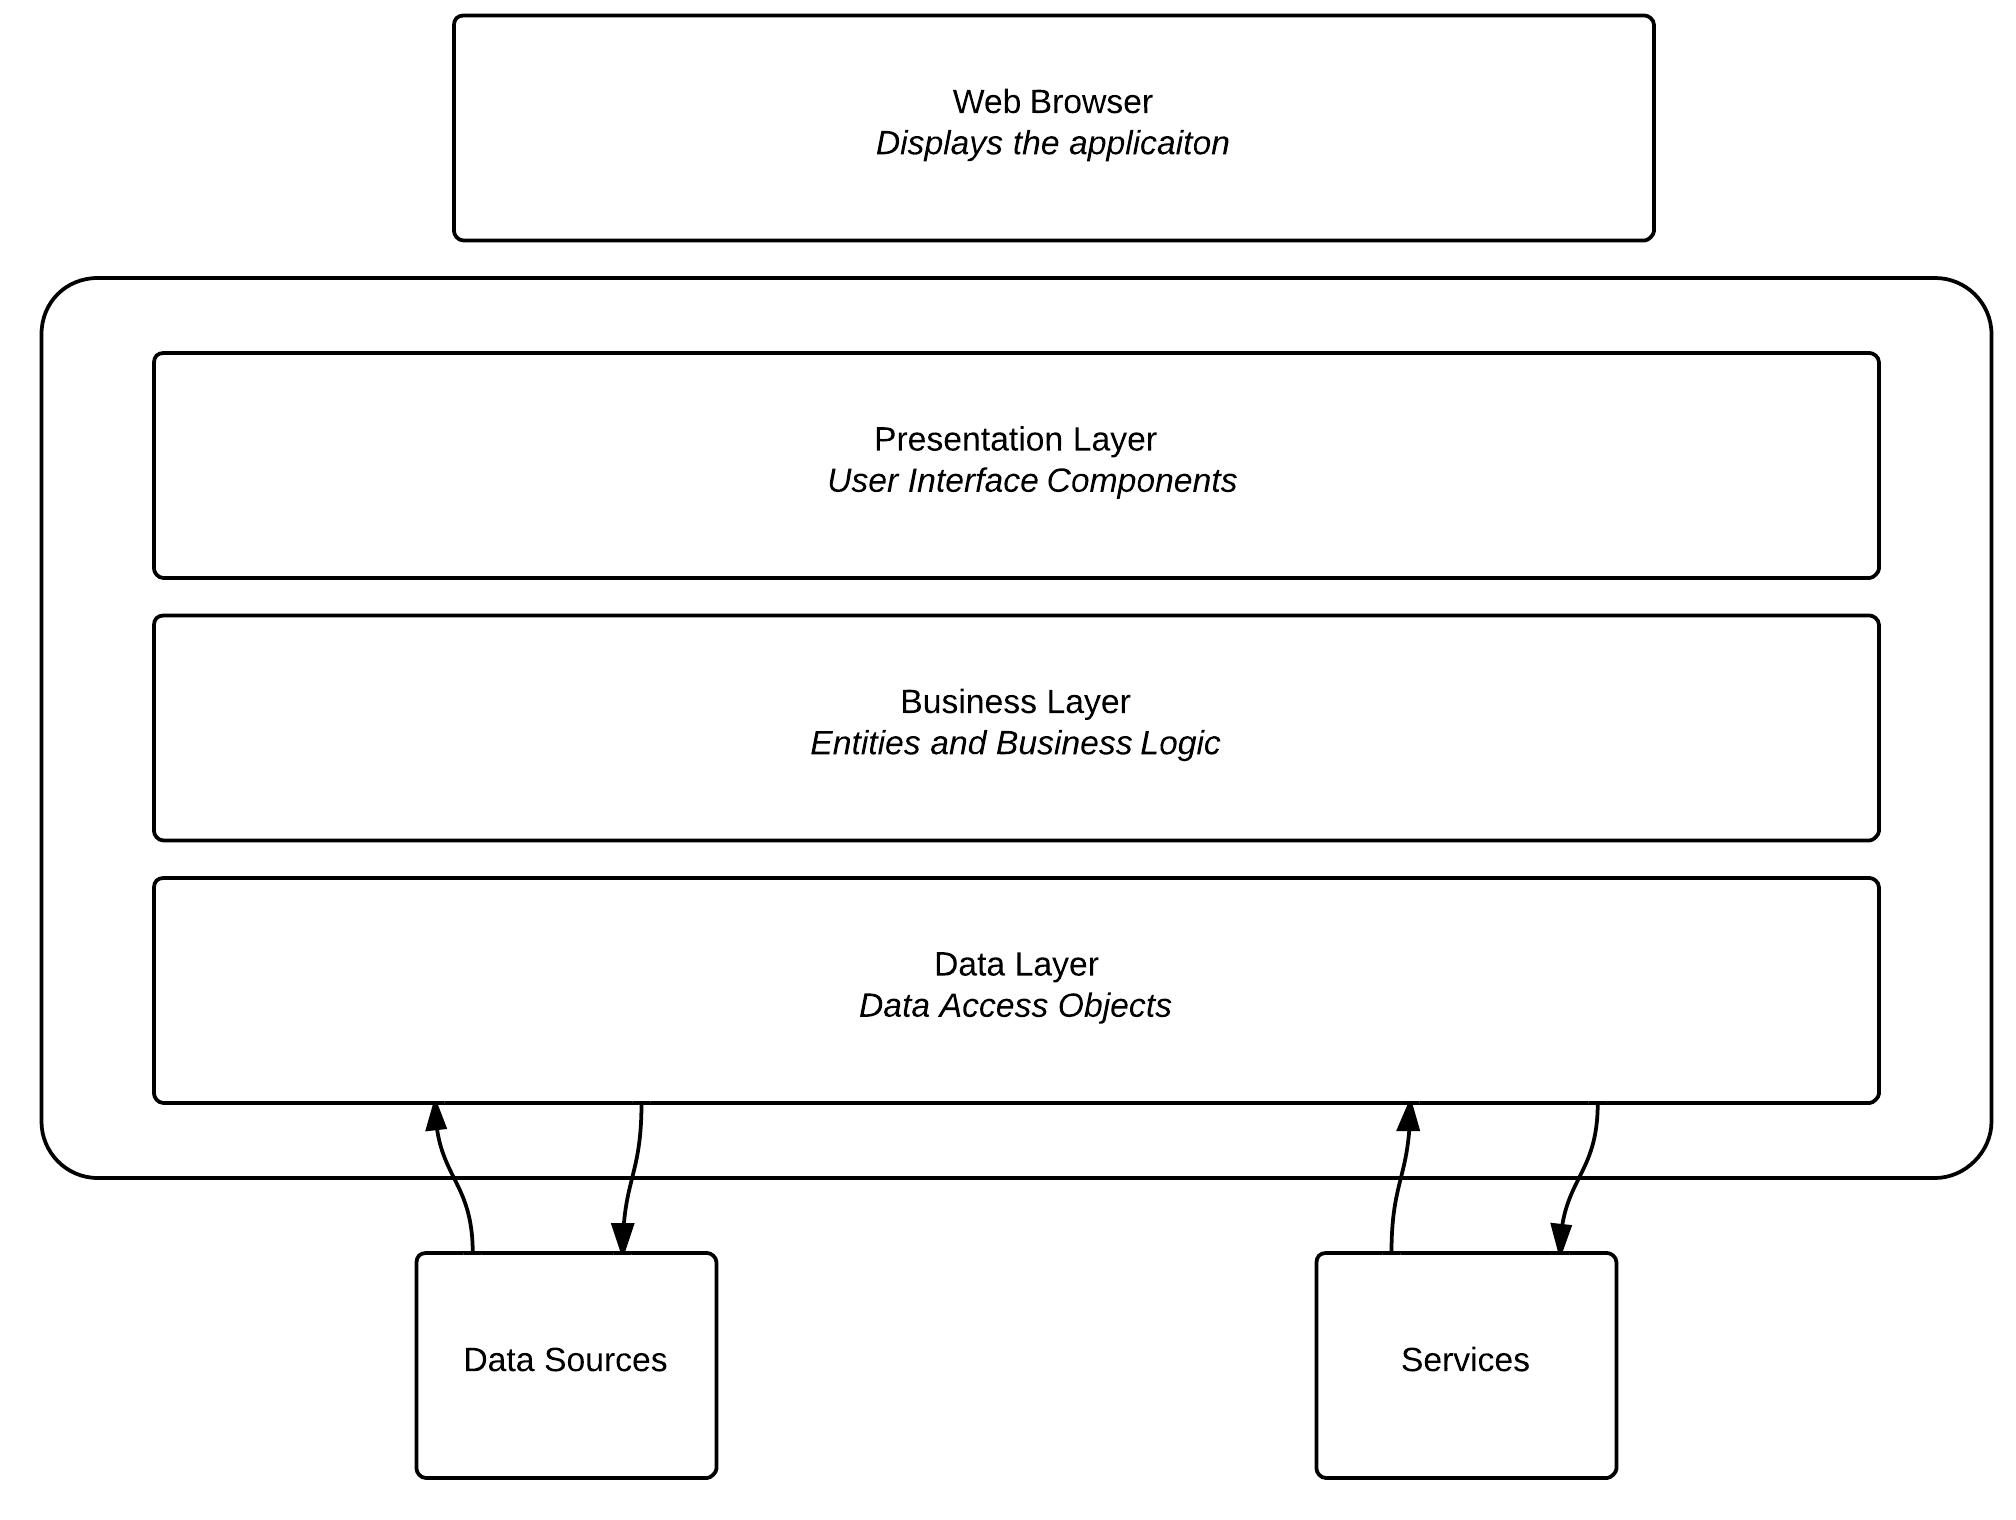
\includegraphics[scale=0.20]{webapp.PNG}
\end{center}
\caption{Typical architecture of a web application}
\label{fig:webarch}
\end{figure}

\begin{figure}[H]
\begin{center}
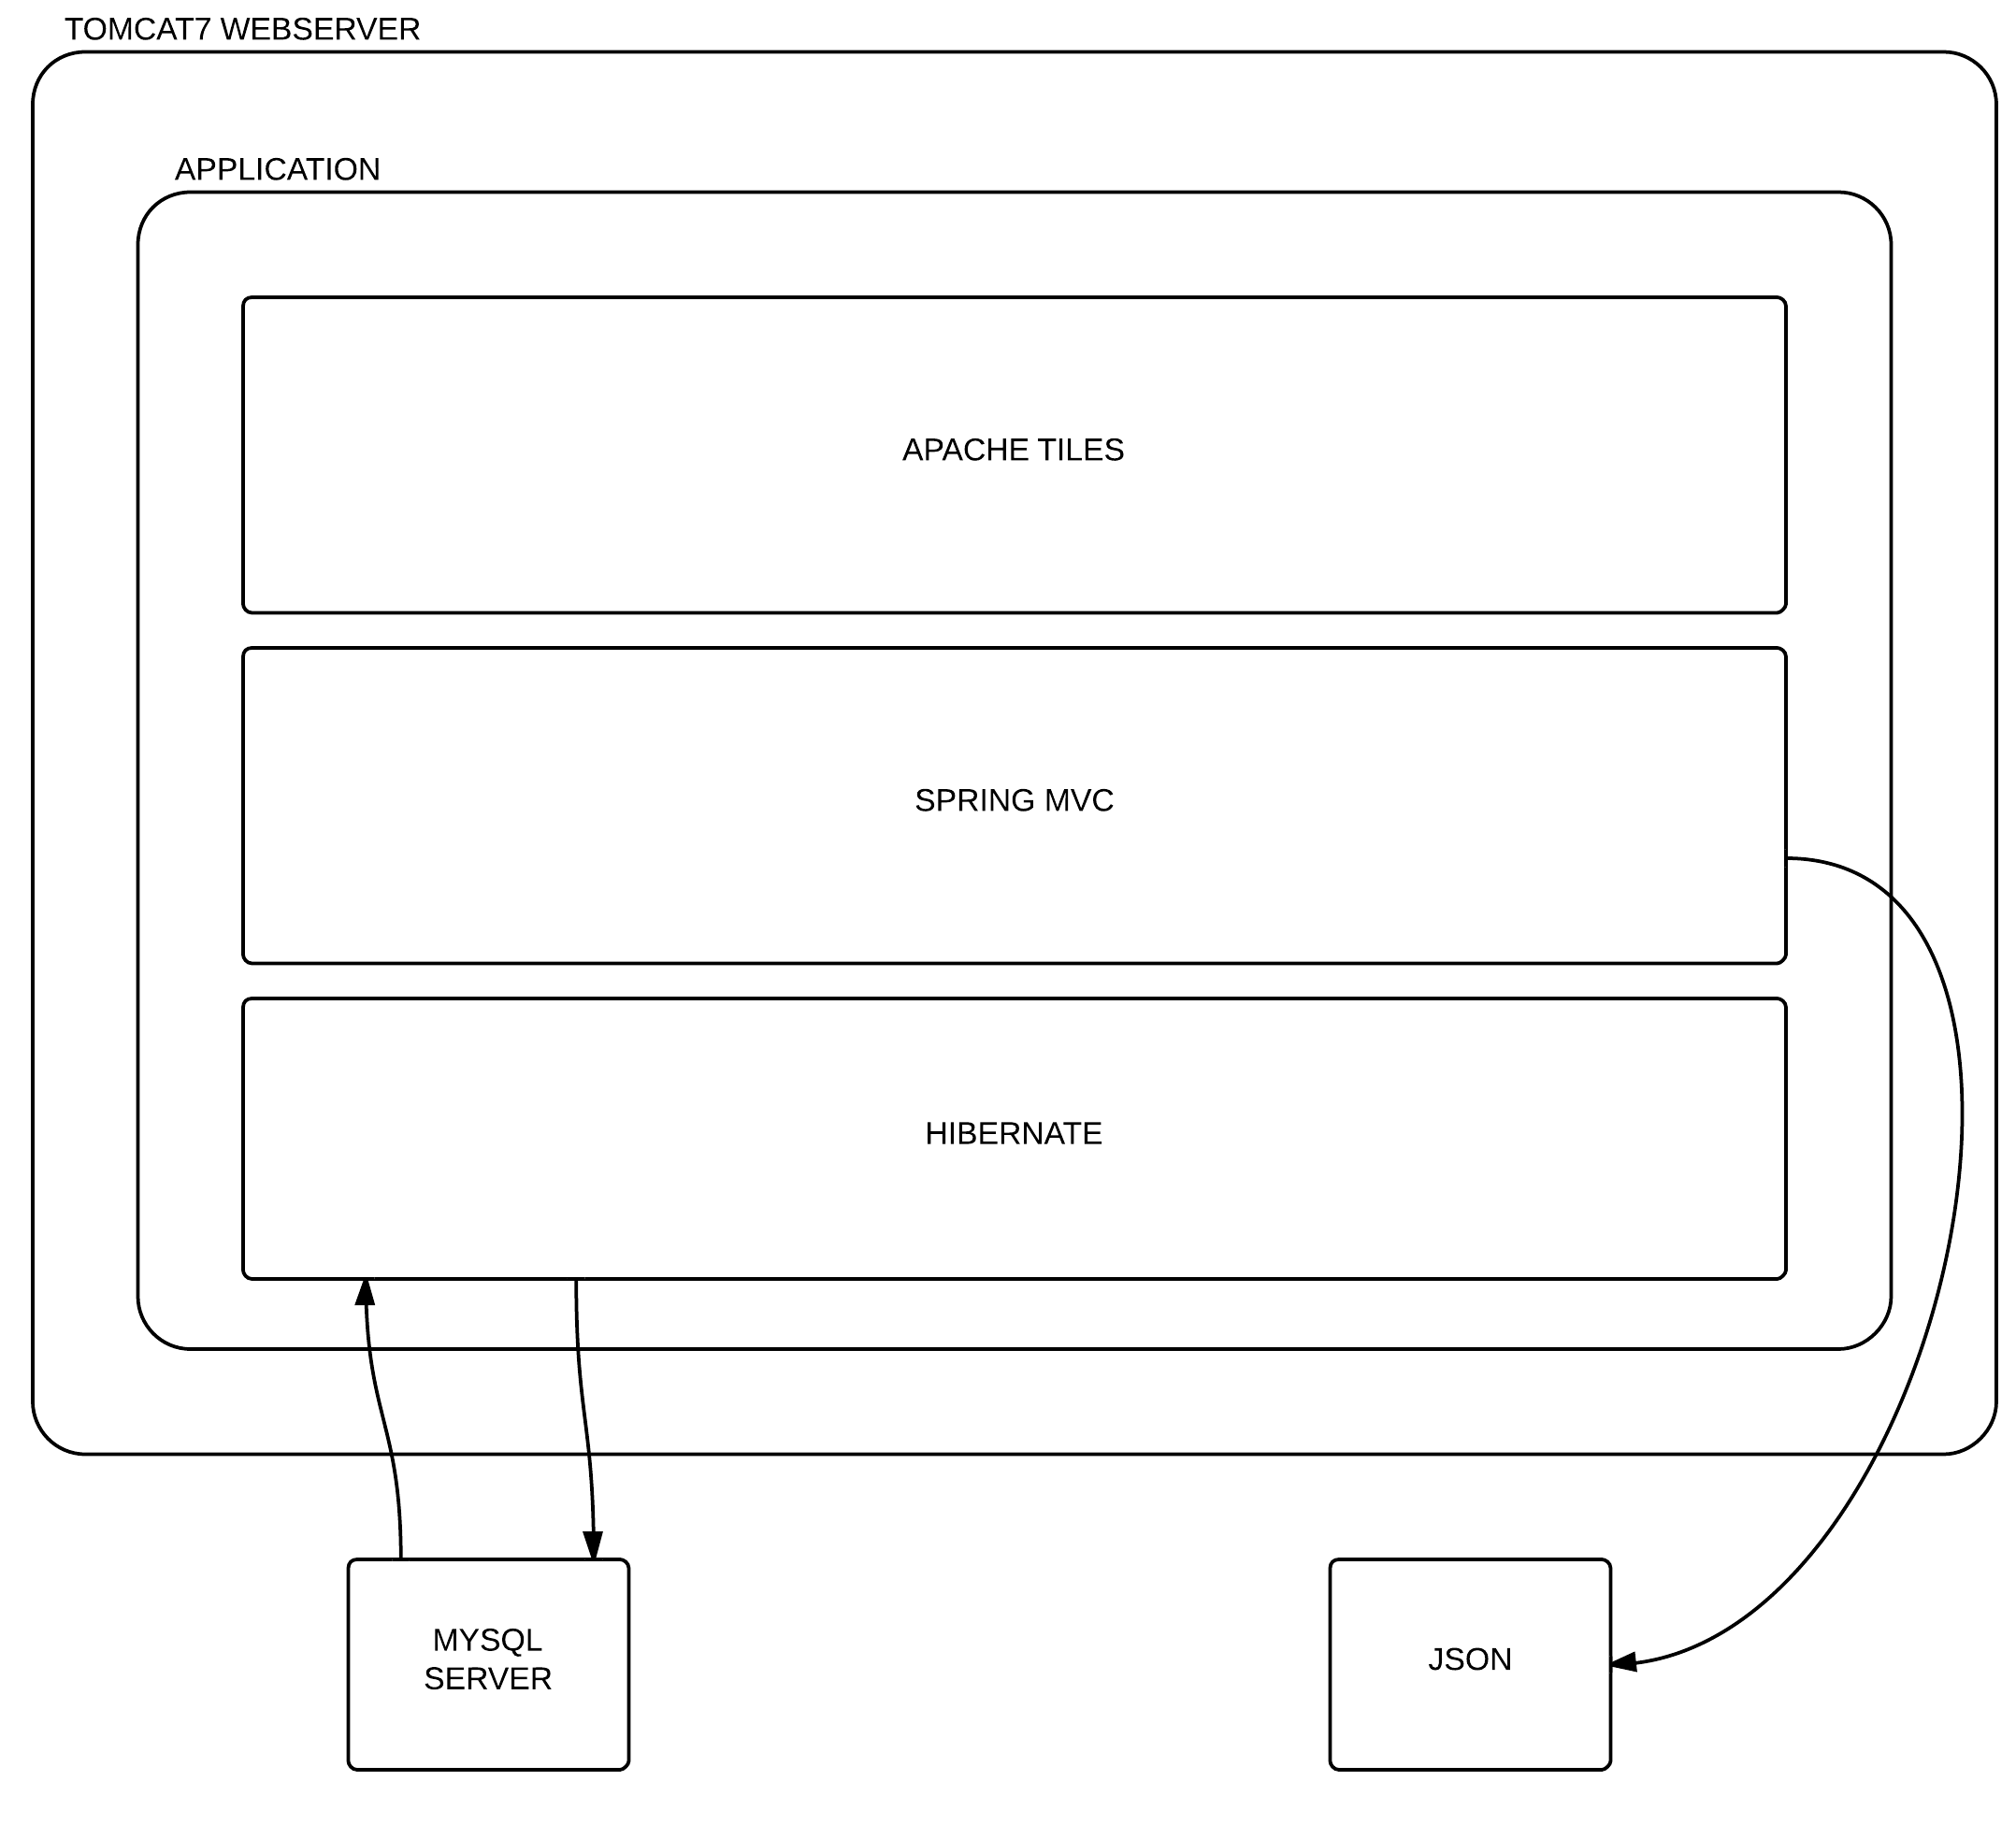
\includegraphics[scale=0.20]{projarch.PNG}
\end{center}
\caption{Architecture of FYP application}
\label{fig:projstack}
\end{figure}

A more common stack within this course is the LAMP, or WAMP, open source solution. This consists of: 

\begin{enumerate}
\item \underline{\textbf{L}}inux or \underline{\textbf{W}}indows
\begin{itemize}
\item The operating system used in the solution
\end{itemize}
\item \underline{\textbf{A}}pache HTTP Server
\begin{itemize}
\item The server used to manage HTTP requests
\end{itemize}
\item \underline{\textbf{M}}y SQL Server
\begin{itemize}
\item The layer responsible for data persistence
\end{itemize}
\item \underline{\textbf{P}}HP, Perl or Python
\begin{itemize}
\item These are scripting languages used for dynamic web pages and web development
\end{itemize}
\end{enumerate}

A large benefit of this stack in the ease of deployment of any application created. The Tralee Tennis Club website seems to have been implemented using this solution.

\section{Objectives}

\subsection{Primary Objectives}

The primary objective of this project is to show the benefits to quality attributes that the use of an architectural stack provides. The architectural stack within this project contains Spring MVC, Hibernate ORM and Apache Tiles. 

This project will examine the support provided for specific quality attributes: Security, Productivity, Extensibility and Performance. The provision of these attributed as provided by these frameworks will be examined, with cognisance of usability. 

\subsection{Secondary Objectives}

The secondary objectives of this project are: 

\begin{itemize}
\item To gain knowledge of the development of a web application using frameworks
\item To obtain experience working with a architectural stack common to industry
\item To use metrics and code visualisations within a project in order to guide and aid development of an application.
\end{itemize}

\section{Scope}

This report, and project, are focused on the effect that frameworks have on quality attributes. As such, the full functionality of the web application is outside the scope of this project. While requirements are an important part of every software life-cycle process, the full methodology for requirements elicitation is outside the scope of this project. Though web services are touched on briefly, they, and mobile viewing, are not important to the overall project, and are not discussed extensively. 

\section{Methodology}

The methodology used for this project was as follows:

\begin{enumerate}
\item Learn the technology
\begin{itemize}
\item The first thing that was examined was the configuration of the technologies needed to implement a web application using Spring, Hibernate and Tiles. As such a set of tutorial videos provided by an educational website called Udemy provided a starting point. The paid videos totalled about 28 hours of content spread over 170 videos.\parencite{udemy}
\end{itemize}
\item Define objectives
\begin{itemize}
\item The next step was to define learning objectives from the project. The decision was made to focus on the support of specific quality attributes by the use of web application frameworks. This is the main objective of the report, with secondary objectives relating to the use of metrics within a development in order to support overall quality of the application.
\end{itemize}
\item Requirements Engineering
\begin{itemize}
\item The elicitation of requirements from key stakeholders was an important step, and ensured that development of the application was in line with the expectations of those eventually utilising the application. Storyboarding, exploratory interviews and focus groups were used to elicit possible functional requirements, and to identify non function requirements key to the application.
\end{itemize}
\item Design
\begin{itemize}
\item The design of the system, such as the structure for user authentication, and the overall design of the application were examined, with cognisance of design patterns. The frameworks used within this application mandate programmers technique, and guide developers towards best practice.
\end{itemize}
\item Implementation, Testing and Deployment
\begin{itemize}
\item Once design of the application was completed, it needed to be implemented. Due to time constraints within a final year project, unit testing and some light user testing were the only techniques available to use. Deployment was a personal goal, as previous project had all been local applications.
\end{itemize}
\item Evaluation
\begin{itemize}
\item Evaluation of the application was performed by comparing the final application to previous work involving security completed in a previous module, Distributed Systems. OWASP was chosen to evaluate the security component of the application. Productivity was examined through a comparative use of both Hibernate and JDBC within one of the Data Access Object (DAO) classes. A performance test was prepared for comparing Hibernate and JDBC. A usability study, based on a framework \parencite{holzinger2005usability}, is also documented and a number of applications evaluated.
\end{itemize}
\end{enumerate}